\documentclass[handout,10pt]{beamer}
\usepackage{SexySlides1,fancyvrb,outlines,pbox}

\definecolor{UniBlue}{RGB}{83,121,170}
\setbeamercolor{title}{fg=UniBlue}
\setbeamercolor{frametitle}{fg=UniBlue}
\newcommand{\colubf}{\color{UniBlue} \bf}

%% smart verbatim
\fvset{framesep=1cm,fontfamily=courier,fontsize=\scriptsize,framerule=.3mm,numbersep=1mm,commandchars=\\\{\}}

\title[Copula network]
{\Large  
Copula-based directional dependence networks for multivariate data
}

\author[Subho Majumdar]
{Subho Majumdar}

\institute[]
{School of Statistics, University of Minnesota} 

\date [May 5, 2014]

%%%%%%%List Outline in the beginning of each section.

%-------------------------------------------------------------------

%%%%%%%List Outline in the beginning of each section.
\AtBeginSection[] {
   \begin{frame}
       \frametitle{Outline}
       \tableofcontents[currentsection]
   \end{frame}
}

%-------------------------------------------------------------------
\begin{document}

%\begin{frame}
 \frame{ \titlepage}
%\end{frame}

\frame{\frametitle{Table of contents}\tableofcontents}

%---------------------------------------------------
\section{Introduction}

\begin{frame}
\frametitle{Background}
\begin{outline}
\1 Copulas model joint dependency structure in financial and survival data.
\2 \textbf{Pros}: Distribution-free: invariant under monotone transformations on data, can model different kinds of tail-dependence
\2 \textbf{Cons}: Multivariate parametric models insufficient
\vspace{.2cm}
\1 \textbf{Copula selection} done by
\2 AIC/BIC \cite{aicbiccop}
\2 minimizing distance to empirical copula function \cite{empcop}
\vspace{.2cm}
\1 \textbf{Multivariate dependency}
\2 Vine copulas provide a conditional pairwise dependency tree, but decomposition of pdf is not unique.
\2 \cite{paircop} did pairwise copula on multivariate genetic data, but no copula selection.
\end{outline}
\end{frame}

\begin{frame}
\frametitle{Overview of work}
\begin{itemize}
\item Derived depth-based (robust?) estimators of copula parameters
\vspace{.2cm}
\item Choose parametric copula families to model different tail dependencies
\vspace{.2cm}
\item Calculate ML or depth-based estimate, choose best-fitting copula
\vspace{.2cm}
\item Repeat for all pairs of variables in multivariate data: gives dependency structure
\vspace{.2cm}
\item Application on two datasets
\vspace{.2cm}
\item Future work
\end{itemize}
\end{frame}

\section{Preliminaries}

\begin{frame}
\frametitle{Copula functions}
\begin{block}{Defnition}
\begin{itemize}
\item $C:[0,1]^2\rightarrow [0,1]$, uniformly distributed marginals
\item (\textbf{Sklar's theorem}) Any bivariate cdf $H$ on random variables $X,Y$, with marginals $F,G$ respectively, there always exists a copula function $C$ s.t.
$$ H(x,y) = C(F(x),G(y)) $$
i.e. $C(u,v) = H(F^{-1}(u), G^{-1}(v))$ for $(u,v)\in[0,1]^2$.
\end{itemize}
\end{block}

Two types of Copula:
\begin{itemize}
\item \textbf{Inplicit copula}- cdf given as an integral, no closed form
\item \textbf{Explicit copula}- cdf has closed form
\end{itemize}
\end{frame}

\begin{frame}
\frametitle{Implicit copula}
\begin{example}
\begin{itemize}
\item \textbf{Gaussian copula}: Copula parameter is $\rho\in[-1,1]$, the correlation coefficient. {\colubf Models low tail-dependency}.
$$ C_\rho(u,v) = \int_{-\infty}^{\Phi^{-1}(u)}\int_{-\infty}^{\Phi^{-1}(v)} \frac{1}{2\pi\sqrt{1-\rho^2}} \exp\left\{-\frac{x^2-2xy+y^2}{2(1-\rho^2)}\right\}dxdy$$

\item \textbf{$t$ copula}: Parameters $\rho\in [-1,1], \nu=$ degree of freedom. {\colubf Jointly heavy-tailed}.
$$ C_{\rho,\nu}(u,v) = \int_{-\infty}^{t_\nu^{-1}(u)}\int_{-\infty}^{t_\nu^{-1}(v)} \frac{1}{2\pi\sqrt{1-\rho^2}} \left\{-\frac{x^2-2xy+y^2}{2(1-\rho^2)}\right\}^{-(\nu+2)/2}dxdy $$

$\nu\geq 30 \equiv$ Gaussian copula.

\end{itemize}
\end{example}
\end{frame}

\begin{frame}
\frametitle{Explicit copula}
\begin{example}
\begin{itemize}
\item \textbf{Clayton copula}: Parameter $\delta\in(0,\infty)$. $\delta\rightarrow 0$ means independence, $\delta\rightarrow\infty$ means perfect dependence. {\colubf Models heavy dependency on left tail}.
$$ C_\delta (u,v) = (u^{-\delta}+v^{-\delta}+1)^{-1/\delta} $$

\item \textbf{Gumbel copula}: Parameter $\delta\in[1,\infty)$. $\delta=1$ means independence, $\delta\rightarrow\infty$ means perfect dependence. {\colubf Models heavy dependency on right tail}.
$$ C_\delta(u,v) = \exp\left[-\left\{(-\log u)^\delta+(-\log v)^\delta\right\}^{1/\delta}\right] $$
\end{itemize}
\end{example}

\textbf{Note}: Both Clayton and Gumbel copulae are used for positive dependence. For negative dependence, $90^\circ$ (or $270^\circ$) rotated versions are used, which have the same expressions for $C_\delta(u,v)$, but $\delta\in(-\infty,0)$ for Clayton and $\in (-\infty,1]$ for Gumbel copula, respectively.
\end{frame}

\begin{frame}
\frametitle{Likelihood depth}
\begin{itemize}
\item Due to \cite{mizera1}\cite{mizera2}. Consider $n$ iid observations from $Z\sim f_\theta$ with $\theta\in\Theta\subset \mathbb{R}^p$, likelihood function $L(\theta,z) = f(\theta,z)$.
\vspace{.2cm}
\item \textbf{Nonfit} A parameter $\theta\in \Theta$ is nonfit wrt data $(z_1,...,z_n)$ when $\exists\quad \theta'\neq \theta\in \Theta$ s.t. $L(\theta',z_i)>L(\theta,z_i)$, or equivalently for log-likelihood: $l_i(\theta')>l_i(\theta)$ for $i=1,,,n$.
\vspace{.2cm}
\item \textbf{Likelihood depth} at $\theta$ is the minimum proportion of observations that need to be deleted from the data to make $\theta$ a nonfit.
\vspace{.2cm}
\item \textbf{Tangent Likelihood depth} Same as likelihood depth under regularity conditions.
$$d_T(\theta,\bfz) = \frac{1}{n}\inf_{u\neq \bf0_p} \#\{i: u^T\nabla l_i(\theta)\leq 0\} $$
\end{itemize}
\end{frame}

\begin{frame}
\frametitle{Maximum Likelihood Depth Estimator (MLDE)}
\begin{itemize}
\item A parameter value (not necessarily unique) that maximizes the likelihood depth over parameter space $\Theta$:
$$ \hat\theta_d \in \argmax_{\theta\in\Theta} d_T(\theta,\bfz) $$

\item Under regularity conditions, depth at each $\theta\in\Theta$ i.e. $d_T(\theta,\bfz)$ converges uniformly to its population analogue $d_T(\theta,P)$, where $P$ is a valid probability measure. Same holds for the point with maximum depth, given it is unique in the population.
\vspace{.2cm}
\item May give biased estimate of true parameter.
\end{itemize}
\end{frame}

\section{Methods}

\begin{frame}
\frametitle{Copula parameter estimation}
\begin{enumerate}
\item Based on Kendall's $\tau$
\vspace{.2cm}
\item {\colbbf Maximum Likelihood estimates}
\vspace{.2cm}
\item {\colbbf Unbiased estimate based on Max. likelihood depth}
\end{enumerate}
\end{frame}

\begin{frame}
\frametitle{MLDE for copula parameters}
Provides biased estimates for true parameters. For 4 types of copulas relation between MLDEs and true parameters determined numerically:
\begin{itemize}
\item \textbf{Cubic equation} for Gaussian ($c_3=1.2222, c_2=3.6434, c_1=-1.4215,c_0=0.0004,\rho_0=0.461$) and $t$-copula ($c_0,c_1,c_2,c_3,\rho_0$ depend on df $\nu$):
$$ \rho = \begin{cases}
\sign(\hat\rho_d)\left[c_3|\hat\rho_d|^3 + c_2|\hat\rho_d|^2 + c_1|\hat\rho_d| + c_0\right]
&\mbox{if } |\hat\rho_d| > \rho_0\\ 0 &\mbox{if }|\hat\rho_d| \leq \rho_0 
\end{cases}$$
\item \textbf{Linear equation} for Clayton ($a_0=-0.5302, a_1=0.7163$) and Gumbel copula ($a_0=0.02, a_1=0.706$):
$$ \delta = a_0 +a_1\hat\delta_d $$
\end{itemize}
\end{frame}

\begin{frame}
\begin{figure}[t]
	\centering
		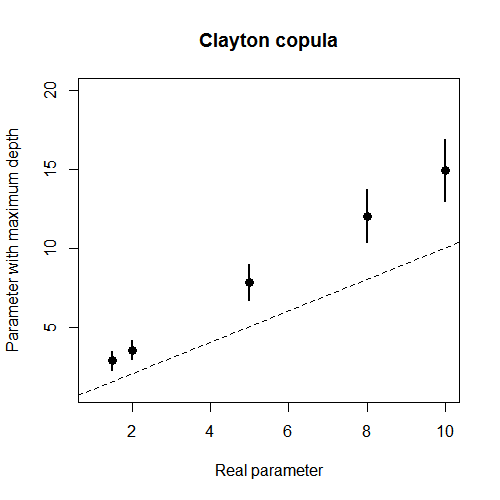
\includegraphics[height=6cm]{CopDepth_Clay.png}
		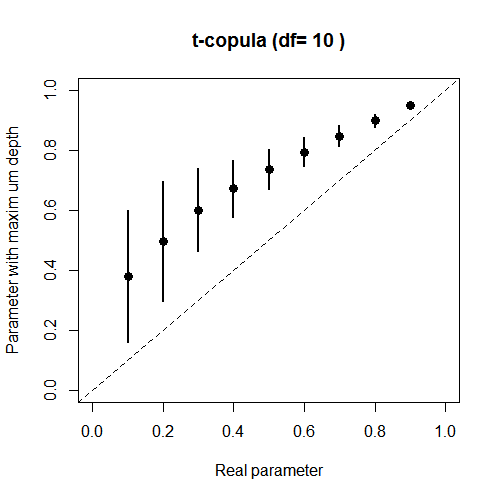
\includegraphics[height=6cm]{CopDepth_t10.png}
	\label{fig:fig1}
	\caption{Mean and standard deviations of simulated parameters with max depth}
\end{figure}
\end{frame}

\begin{frame}
\frametitle{Copula selection}
\begin{itemize}
\item \textbf{Empirical copula} For data $\bfZ_1,...,\bfZ_n$ with $\bfZ_i=(X_i,Y_i)$
$$ C_e(u,v) = \frac{1}{n}\sum_{i=1}^n I(U_i\leq u, V_i\leq v)$$
where $\bfU = F_n(\bfX), \bfV = G_n(\bfY)$ are pseudosamples obtained from the data using marginal empirical distributions $F_n, G_n$ respectively.
\vspace{.2cm}
\item Euclidean distance of a copula $C$ from empirical copula:
$$ d(C,C_e) = \sqrt{\sum_{i=1}^n\sum_{j=1}^n \left[C\left(\frac{i}{n},\frac{j}{n}\right) - C_e\left(\frac{i}{n},\frac{j}{n}\right)\right]^2} $$
\item For the four of copula families, estimate parameters by ML or depth-based method, then choose the copula that minimizes the above distance.
\end{itemize}
\end{frame}

\begin{frame}
\frametitle{Constructing the graph}
\begin{enumerate}
\item Test for independence between a variable pair using test based on asymptotic normality of Kendall's $\tau$ ($n$ = sample size):
$$ \hat\tau \sim AN\left(0,\frac{2(2n+5)}{9n(n-1)}\right) $$
\item Apply algorithm on next page.
\vspace{.2cm}
\item At the end of the algorithm we end up with two graphs, $\bfC_M$ and $\bfC_D$, giving best-fitting copulae, obtained by the two respective methods, for each pair of variables.
\end{enumerate}
\end{frame}

\begin{frame}
\begin{figure}[t]
	\centering
		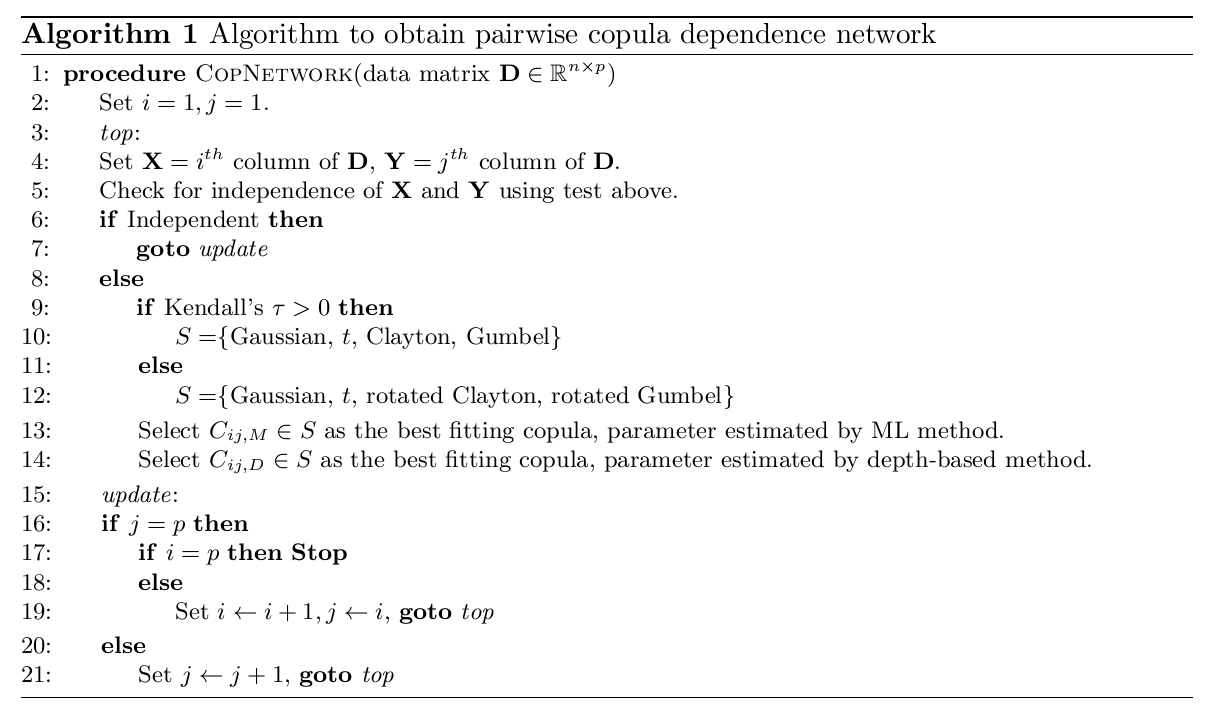
\includegraphics[height=7cm]{algopic.png}
	\label{fig:fig2}
\end{figure}
\end{frame}

\section{Data examples}
\begin{frame}
\frametitle{Data example: Breast Cancer data}
\begin{itemize}
\item From UCI Machine Learning Reopsitory: \url{https://archive.ics.uci.edu/ml/datasets/Breast+Tissue}
\item Impedance measurements from 106 breast tissue samples.
\item 9 measurement variables (I0, PA500, HFS, DA, Area, A/DA, Max IP, DR, P) and a class variable specifying the class of Breast Cancer the patient has (6 or 4 classes).
\end{itemize}
\begin{scriptsize}
\begin{table}[h]\centering
    \begin{tabular}{l|l}
    \hline
    Variable name & Description          \\\hline
    I0       & Impedivity (ohm) at zero frequency                                \\
    PA500    & Phase angle at 500 KHz                                            \\
    HFS      & High-frequency slope of phase angle                               \\
    DA       & Impedance distance between spectral ends                          \\
    AREA     & Area under spectrum                                               \\
    A/DA     & Area normalized by DA                                             \\
    MAX IP   & Maximum of the spectrum                                           \\
    DR       & Distance between I0 and real part of the maximum frequency point  \\
    P        & Length of the spectral curve                                      \\\hline
    \end{tabular}
    \caption{Description of measurement variables in Breast Cancer data}
\end{table}
\end{scriptsize}
\end{frame}

\begin{frame}
\frametitle{Breast Cancer data: analysis}
\begin{itemize}
\item We ignore the class variable due to small sample sizes in each class and obtain the networks from the measurement variables only.
\vspace{.2cm}
\item 28 significantly dependent variable pairs among 36 possible ones.
\vspace{.2cm}
\item Variables except the two phase angle related variables: HFS and PA500, are all dependent on one another.
\vspace{.2cm}
\item Most of these dependencies are symmetric, and  heavy-tailed ($t$-copula) as per the ML method, but light-tailed as per the depth-based method.
\end{itemize}
\end{frame}

\begin{frame}
\frametitle{Breast Cancer data: networks}
\begin{figure}[t]
	\centering
		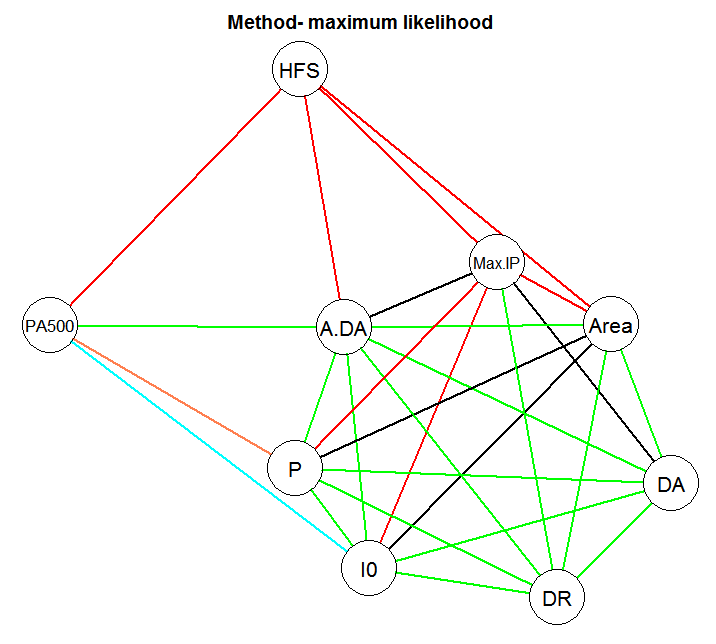
\includegraphics[height=5cm]{cancer_graph_ml.png}
		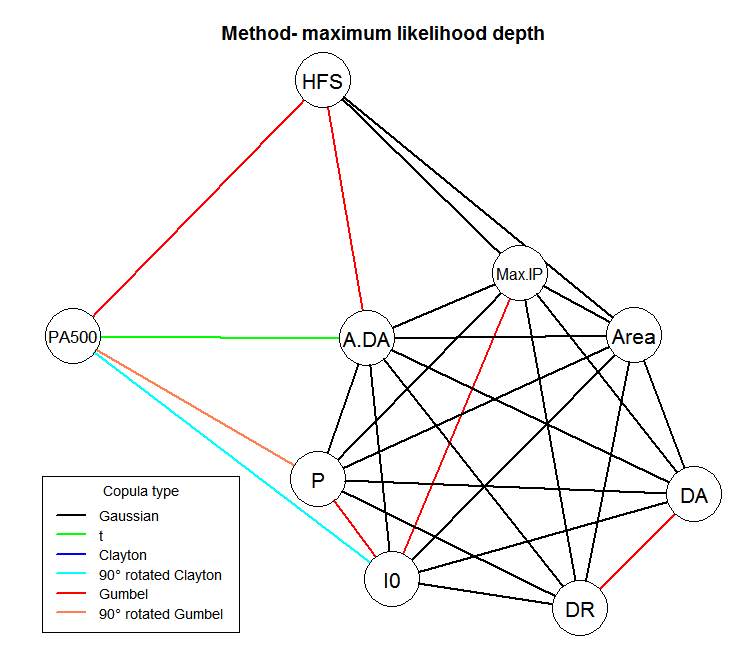
\includegraphics[height=5cm]{cancer_graph_md.png}
	\label{fig:fig2}
	\caption{Graph of Breast Cancer variables obtained by best-fitting (top) ML copula, (Bottom) MLD copula}
\end{figure}
\end{frame}

\begin{frame}
\frametitle{Data example: Cardiotocography (CTG) data}
\begin{itemize}
\item Measurements relating to 2126 fetal cardiotocograms: \url{https://archive.ics.uci.edu/ml/datasets/Cardiotocography}
\vspace{.2cm}
\item 21 predictor variables: Variables 1-7 give numerical measurements (grp A), 8-11 are about variability of cardiograms with respect to time (grp B), Variables 12-21 give measurements of heart-rate histograms (grp C).
\vspace{.2cm}
\item DS, the sixth variable has most of its values set at 0, so we exclude it from our analysis.
\end{itemize}
\end{frame}

\begin{frame}
\frametitle{CTG data: Variable group-specific analysis}
\begin{itemize}
\item Over 90\% of connections between the 20 variables (176 among 190 possible) found significant in the initial screening for dependence.
\item Instead of plotting the graph we analyze the dependence structures within and between the 3 variable groups.
\item 3 within-group ($AA, BB, CC$) and 3 between-group ($AB, AC, BC$) interactions.
\end{itemize}
\begin{scriptsize}
\begin{table}[ht]\centering
    \begin{tabular}{|c||c|c|c|c|c|c|c|}
    \hline
    Interaction & Indep. & Gaussian & $\quad t\quad$ & Clayton & rot. Clayton & Gumbel & rot. Gumbel \\ \hline
    AA                  & 2           & 0        & 0 & 7       & 1               & 0      & 5              \\
    BB                  & 1           & 2        & 1 & 0       & 1               & 0      & 1              \\
    CC                  & 2           & 11       & 9 & 2       & 7               & 5      & 9              \\ \hline\hline
    AB                  & 1           & 4        & 3 & 2       & 11              & 1      & 2              \\
    AC                  & 3           & 16       & 2 & 16      & 18              & 2      & 3              \\
    BC                  & 5           & 7        & 3 & 7       & 11              & 2      & 5              \\ \hline
    \end{tabular}
    \caption{Summary of best-fitting copulae for within (Top 3) and between (bottom 3) group dependencies in CTG data}
\end{table}
\end{scriptsize}
\end{frame}

\begin{frame}
\frametitle{CTG data: Dependence structure for different fetal classes}
\begin{itemize}
\item Within-group dependencies for the 3 fetal classes are also compared.
\item Networks are plotted for groups A and B in 3 sample classes.
\item For variable group C, the summary of copulae fit between the 45 variable-pairs is summarized in table below. Highlights include a high amount of independence in suspect class and high asymmetric dependencies in pathologic class.
\end{itemize}
\begin{scriptsize}
\begin{table}[h]\centering
    \begin{tabular}{|c||c|c|c|c|c|c|c|}
    \hline
    Sample class & Indep. & Gaussian & $\quad t\quad$ & Clayton & rot. Clayton & Gumbel & rot. Gumbel \\ \hline
    Normal & 4 & 13 & 8 & 4 & 5 & 7 & 4 \\
    Suspect & 11 & 8 & 8 & 3 & 3 & 10 & 2 \\
    Pathologic & 3 & 9 & 2 & 2 & 11 & 7 & 11 \\ \hline
    \end{tabular}
    \caption{Best-fitting copulae by ML method for group C variables in CTG data}
\end{table}
\end{scriptsize}
\end{frame}

\begin{frame}
\frametitle{CTG data: networks}
\begin{figure}[t]
	\centering
		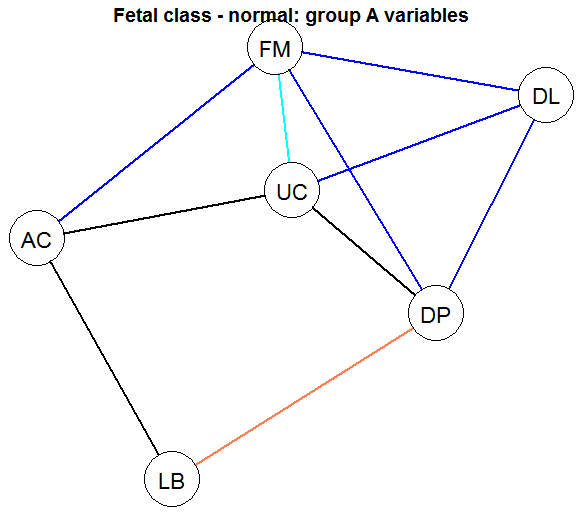
\includegraphics[height=3.5cm]{ctgplot_1a.png}
		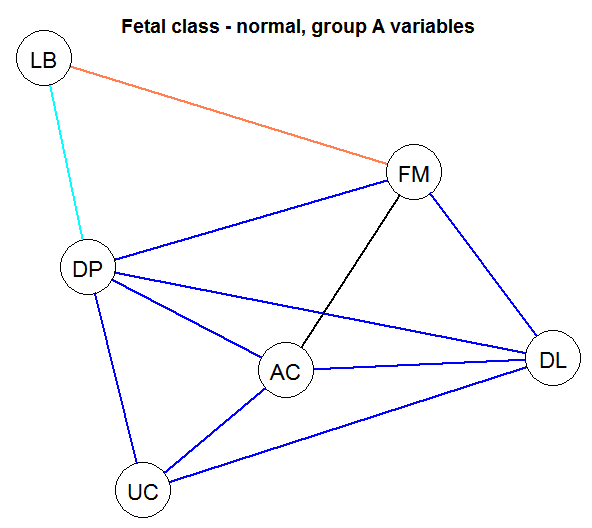
\includegraphics[height=3.5cm]{ctgplot_2a.png}
		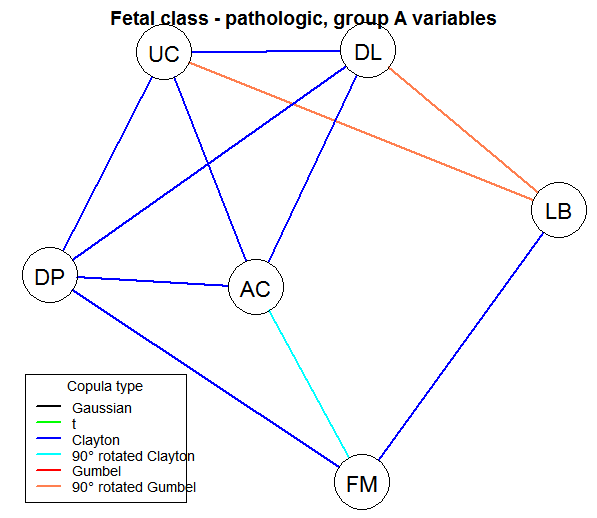
\includegraphics[height=3.5cm]{ctgplot_3a.png}
	\label{fig:fig2}
	\caption{Graph of group A variables for 3 classes}
\end{figure}
\end{frame}

\begin{frame}
\frametitle{CTG data: networks}
\begin{figure}[t]
	\centering
		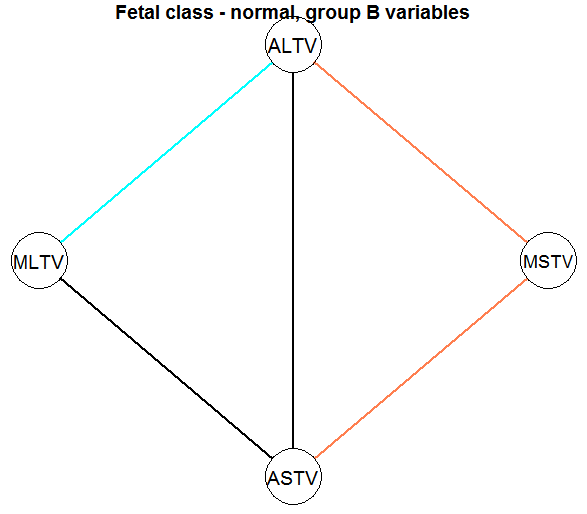
\includegraphics[height=3.5cm]{ctgplot_1b.png}
		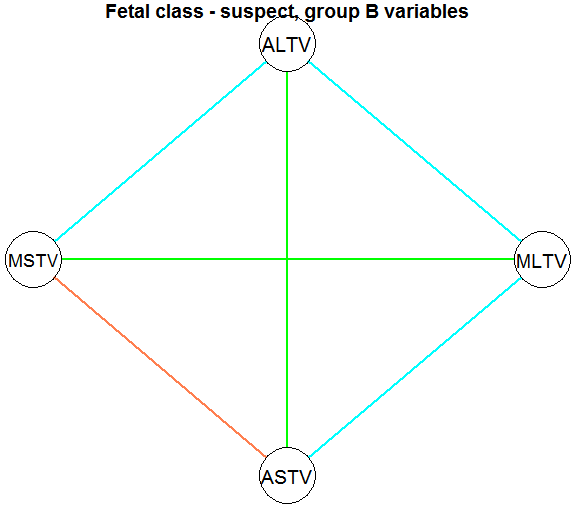
\includegraphics[height=3.5cm]{ctgplot_2b.png}
		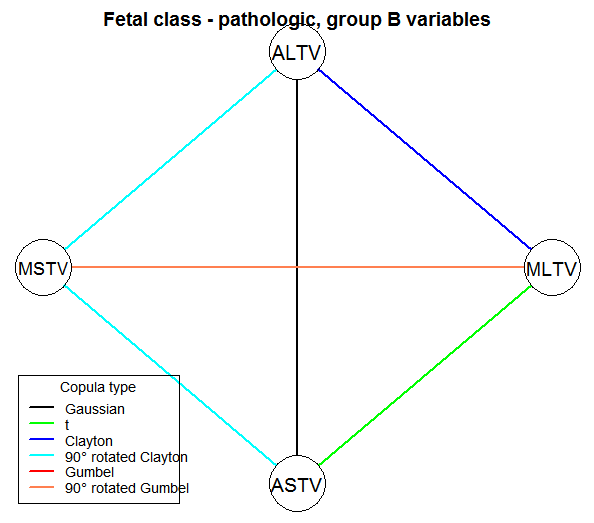
\includegraphics[height=3.5cm]{ctgplot_3b.png}
	\label{fig:fig2}
	\caption{Graph of group B variables for 3 classes}
\end{figure}
\end{frame}

\begin{frame}
\frametitle{Summary and future work}
\begin{itemize}
\item Formulation of a distribution-free method to analyze the nature of dependencies between pairs of variables in a multivariate dataset.
\item Application on two real datasets\\
\vspace{.5cm}
Future works include:
\item \textbf{Using conditional bivariate copula} for each variable-pair to eliminate effect of other variables
\item \textbf{Detailed simulation studies} to compare between the two methods of copula parameter estimation
\item \textbf{Analyze genetic data} and compare the methodology with other known methods
\end{itemize}
\end{frame}

\begin{frame}
\frametitle{Acknowledgement}
I thank my adviser Prof. Snigdhansu Chatterjee for his guidance and valuable inputs throughout the project.
\end{frame}

\begin{frame}
\frametitle{References}
\bibliographystyle{acm}
\bibliography{depth}
\end{frame}

\begin{frame}
\centering\huge
\textcolor{UniBlue}{\textbf{THANK YOU!}}
\end{frame}

\end{document} 

